%% -*- coding: utf-8 -*-
\documentclass[12pt,a4paper]{scrartcl} 
\usepackage[utf8]{inputenc}
\usepackage[english,russian]{babel}
\usepackage{indentfirst}
\usepackage{misccorr}
\usepackage{graphicx}
\usepackage{amsmath}
\begin{document}
	\begin{titlepage}
		\begin{center}
			\large
			МИНИСТЕРСТВО НАУКИ И ВЫСШЕГО ОБРАЗОВАНИЯ РОССИЙСКОЙ ФЕДЕРАЦИИ
			
			Федеральное государственное бюджетное образовательное учреждение высшего образования
			
			\textbf{АДЫГЕЙСКИЙ ГОСУДАРСТВЕННЫЙ УНИВЕРСИТЕТ}
			\vspace{0.25cm}
			
			Инженерно-физический факультет
			
			Кафедра автоматизированных систем обработки информации и управления
			\vfill

			\vfill
			
			\textsc{Отчет по практике}\\[5mm]
			
			{\LARGE \textit{Программный модуль анализа метеоданных с использованием методов искусственного интеллекта}}
			\bigskip
			
			2 курс, группа 2УТС
		\end{center}
		\vfill
		
		\newlength{\ML}
		\settowidth{\ML}{«\underline{\hspace{0.7cm}}» \underline{\hspace{2cm}}}
		\hfill\begin{minipage}{0.5\textwidth}
			Выполнил:\\
			\underline{\hspace{\ML}} К.\,А.~Кузьмин\\
			«\underline{\hspace{0.7cm}}» \underline{\hspace{2cm}} 2022 г.
		\end{minipage}%
		\bigskip
		
		\hfill\begin{minipage}{0.5\textwidth}
			Руководитель:\\
			\underline{\hspace{\ML}} С.\,В.~Теплоухов\\
			«\underline{\hspace{0.7cm}}» \underline{\hspace{2cm}} 2022 г.
		\end{minipage}%
		\vfill
		
		\begin{center}
			Майкоп, 2022 г.
		\end{center}
	\end{titlepage}
	
	\section{Введение}
	\label{sec:intro}
	
	В настоящее время особенно актуальными являются вопросы качественного анализа данных в процессе принятия решений в различных областях. Одними из особенно важных показателей являются метеоданные, то есть данные о погодных условиях в конкретной местности в определенное время. В связи с этим, актуальным является разработка программного решения, которое позволит получать метеоданные, а также осуществлять их дальнейший анализ с применением методов искусственного интеллекта.
	
	\begin{enumerate}
	\item Текстовая формулировка задачи:
	
	Написать программу для анализа метеоданных с использованием методов искусственного интеллекта
	\item Пример кода, решающего данную задачу приведен в пункте~\ref{sec:exp:code} на стр.~\pageref{sec:exp:code}
	\item Результат работы программы представлен в пункте~\ref{sec:result:screen} на стр.~\pageref{sec:result:screen}
	\end{enumerate}
	
	\section{Ход работы}
	\label{sec:exp}
	
	\subsection{Код программы}
	\label{sec:exp:code}
	\begin{verbatim}
	# Подготовка данных
	df = pd.read_csv('weather.csv')
	df = df.drop(['P','Pa','ff10','ff3','N','WW','W1','W2','Tn','Tx',
	'Cl','Nh','H','Cm','Ch','VV','Td','tR','E','Tg','E\'','sss'],axis=1)
	le = LabelEncoder()
	le.fit(df['DD'])
	df['DD'] = le.transform(df['DD'])
	df.loc[(df.RRR == 'Осадков нет'), 'RRR'] = 0.0
	df.loc[(df.RRR == 'Следы осадков'), 'RRR'] = 0.0
	df['RRR'] = df['RRR'].fillna(df['RRR'].median())
	df["RRR"] = pd.to_numeric(df["RRR"], downcast="float")
	df['Po'] = le.fit_transform(df['Po'])
	df['U'] = le.fit_transform(df['U'])
	
	# Разделение выборки
	df.to_csv('weather.csv',index=False)
	x_train, x_test, y_train, y_test = train_test_split(df[['T', 'Po',
	'U', 'DD', 'RRR']], df['Ff'], test_size=0.3, random_state=1)
	
	# Нормализация
	std = StandardScaler()
	df['DD'] = pd.DataFrame(std.fit_transform(df[['DD']]))
	
	# Линейная многофакторная регрессия
	reg = LinearRegression().fit(x_train, y_train)
	print(reg.score(x_test, y_test))
	print(reg.coef_)
	print(reg.intercept_)
	reg.predict(x_test)
	fig, ax = plt.subplots()
	plt.rcParams['figure.figsize'] = [5, 3]
	ax.plot(range(1,len(y_test)+1), y_test, 'r-',
	range(1,len(y_test)+1), reg.predict(x_test), 'g-')
	plt.show()
	
	# Дерево решений
	params = {'max_depth' : np.arange(1,15,1), 'min_samples_leaf' :
	range(1,15,1)}
	clf = tree.DecisionTreeRegressor(random_state=1)
	grid_clf = GridSearchCV(clf, params, cv=5, n_jobs=-1)
	grid_clf.fit(x_train, y_train)
	print(grid_clf.best_params_)
	best_cls = grid_clf.best_estimator_
	y_pred = best_cls.predict(x_test)
	print(mean_absolute_percentage_error(y_test, y_pred))
	print(grid_clf.best_score_)
	fig, ax = plt.subplots()
	plt.rcParams['figure.figsize'] = [5, 3]
	ax.plot(range(1,len(y_test)+1), y_test, 'r-',
	range(1,len(y_test)+1), best_cls.predict(x_test), 'g-')
	plt.show()
	
	# Многослойный полносвязный персептрон
	regr = MLPRegressor(random_state=1, max_iter=500,
	solver='lbfgs').fit(x_train, y_train)
	fig, ax = plt.subplots()
	plt.rcParams['figure.figsize'] = [5, 3]
	ax.plot(range(1,len(y_test)+1), y_test, 'r-',
	range(1,len(y_test)+1), regr.predict(x_test), 'g-')
	plt.show()
	
	\end{verbatim}
	
	\section{Результат работы программы}
	\label{sec:result}
	
	\subsection{Графики}
	\label{sec:result:screen}
	\begin{figure}[h]
	\centering
	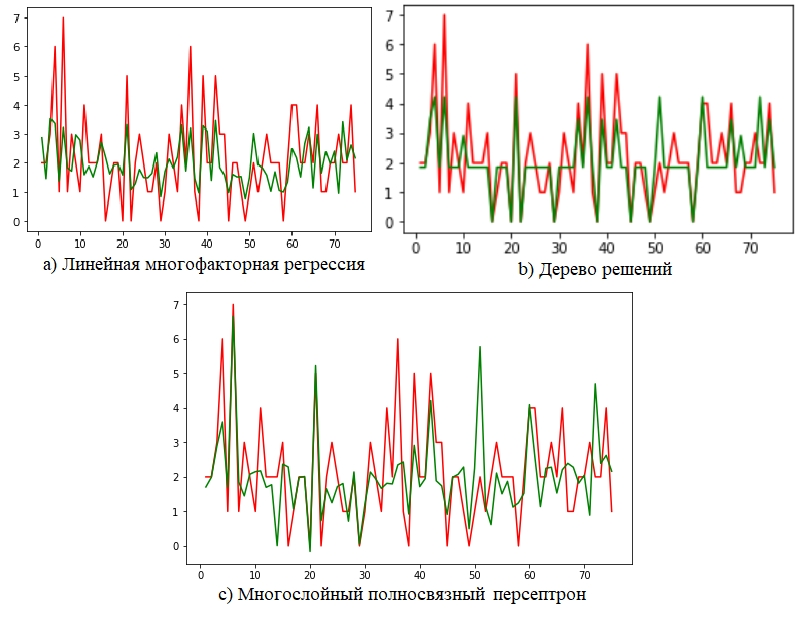
\includegraphics[width=1\textwidth]{result.jpg}
	\caption{Графики}\label{figure:screen}
	\end{figure}

	\begin{thebibliography}{9}
	\bibitem{Knuth-2003}Кнут Д.Э. Всё про \TeX. \newblock --- Москва: Изд. Вильямс, 2003 г. 550~с.
	\bibitem{Lvovsky-2003}Львовский С.М. Набор и верстка в системе \LaTeX{}. \newblock --- 3-е издание, исправленное и дополненное, 2003 г.
	\bibitem{Voroncov-2005}Воронцов К.В. \LaTeX{} в примерах. 2005 г.
	\bibitem{Muller-2019}Мюллер Д.П. Python для чайников. Москва, Санкт-Петербург: Изд. Диалектика, 2019 г.
	\bibitem{Elbon-2019}Крис Элбон. Машинное обучение с использованием Python. Сборник рецептов. Санкт-Петербург: Изд. БХВ-Петербург, 2019 г.
	\bibitem{Rashka-2017}Себастьян Рашка. Python и машинное обучение. Москва: Изд. ДМК Пресс, 2017 г.
	\end{thebibliography}
	
\end{document}
